In this chapter we present the guidelines of designing a PREcision Timed (PRET) Machine. 
It is important to understand why and how current architectures fall short of timing predictability and repeatability.
Thus, we first discuss common architectural designs and their effects on execution time, and point out some key issues and trade-offs when designing architectures for predictable and repeatable timing.

\section{Pipelines}
The introduction of pipelining vastly improved the average-case performance of programs.
It allows faster clock speeds, and improves instruction throughput compared to single cycle architectures.
Pipelining begin executing subsequent instructions while prior instructions are still in execution. 
Ideally each processor cycle one instruction completes and leaves the pipeline as another enters and begins execution. 
In reality, different pipeline hazards occur which reduce the throughput and create stalls in the pipeline.
Different techniques were introduced to handle the effects of pipeline hazards, and greatly effect to the timing predictability and repeatability of an architecture.     
To illustrate this point, we discuss some basic hardware additions proposed to reduce performance penalty from hazards, and show how they effect the execution time and predictability. 

\subsection{Pipeline Hazards}
\begin{wrapfigure}{r}{0.5\textwidth}
  \vspace{-20pt}
  \begin{center}
    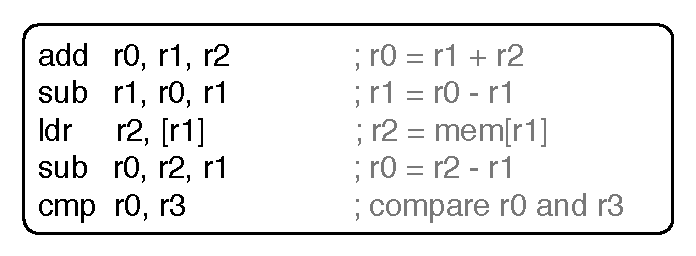
\includegraphics[scale=.65]{figs/sample_data_dependent_code}
  \end{center}
  \vspace{-20pt}
  \caption{Sample code with data dependencies}
  \label{fig:sample_data_dependent_code}
\end{wrapfigure}
Data hazards occur when instructions need the results of previous instructions that have not yet committed.
The code segment shown in figure~\ref{fig:sample_data_dependent_code} contains instructions that each depend on the result of its previous instruction.
Figure~\ref{fig:data_depend_execution_non_interleaved} shows two ways data hazards can be handled in a single-threaded pipeline. 
In the figure, time progresses horizontally towards the right, each time step, or column, represents a processor cycle.
Each row represents an instruction that is fetched and executed within the pipeline.
Each block represents the instruction entering the different stages of the pipeline -- fetch (F), decode (D), execute (E), memory (M) and writeback (W).   
The pipelines here are assumed to have a similar design to the five stage pipeline mentioned in Hennessy and Pattern~\todo{cite hennessy and patterson}.

A simple but effective way of handling data hazards is by simply stalling the pipeline until the previous instruction completes.
% Data hazards in this case are handled by inserting pipeline delays to ensure the completion of all dependent instructions.
%Similar to inserting pipeline delays of control-flow hazards, this method allows for predictable static execution time analysis, but at a slight cost of performance. 
%Figure~\ref{fig:data_depend_execution_non_interleaved} shows the execution of the code segment on pipelines with and without forwarding.
This is shown in the top of figure~\ref{fig:data_depend_execution_non_interleaved}. 
Pipeline delays (or bubbles) are inserted for instructions to wait until the previous instruction is complete.
The dependencies between instructions are shown in the figure to make clear why the pipeline bubbles are necessary.
The performance penalty incurred in this case is the pipeline delays inserted to wait for the previous instruction to complete.
Data forwarding was introduced to remove the need for inserting bubbles into the pipeline.
Data forwarding relies on the fact that the results of the previous instruction is typically available before the it commits.  
%Data forwarding is the most common way of handling data hazards that occur from pipelining.  
A data forwarding circuitry consists of backwards paths for data from later pipeline stages to the inputs of earlier pipeline stages, and multiplexers to select amongst all data signals. 
Because it provides a way to directly access computation results from the previous instruction before the previous instruction finishes, it removes the need to wait for the previous instruction to commit.  
The pipeline controller dynamically detects whether a data-dependency exists, and changes the selection bits to the multiplexers accordingly so the correct operands are selected.
The bottom of figure~\ref{fig:data_depend_execution_non_interleaved} shows the execution with forwarding in the pipeline.
\begin{figure}
\vspace{-20pt}
\begin{center}
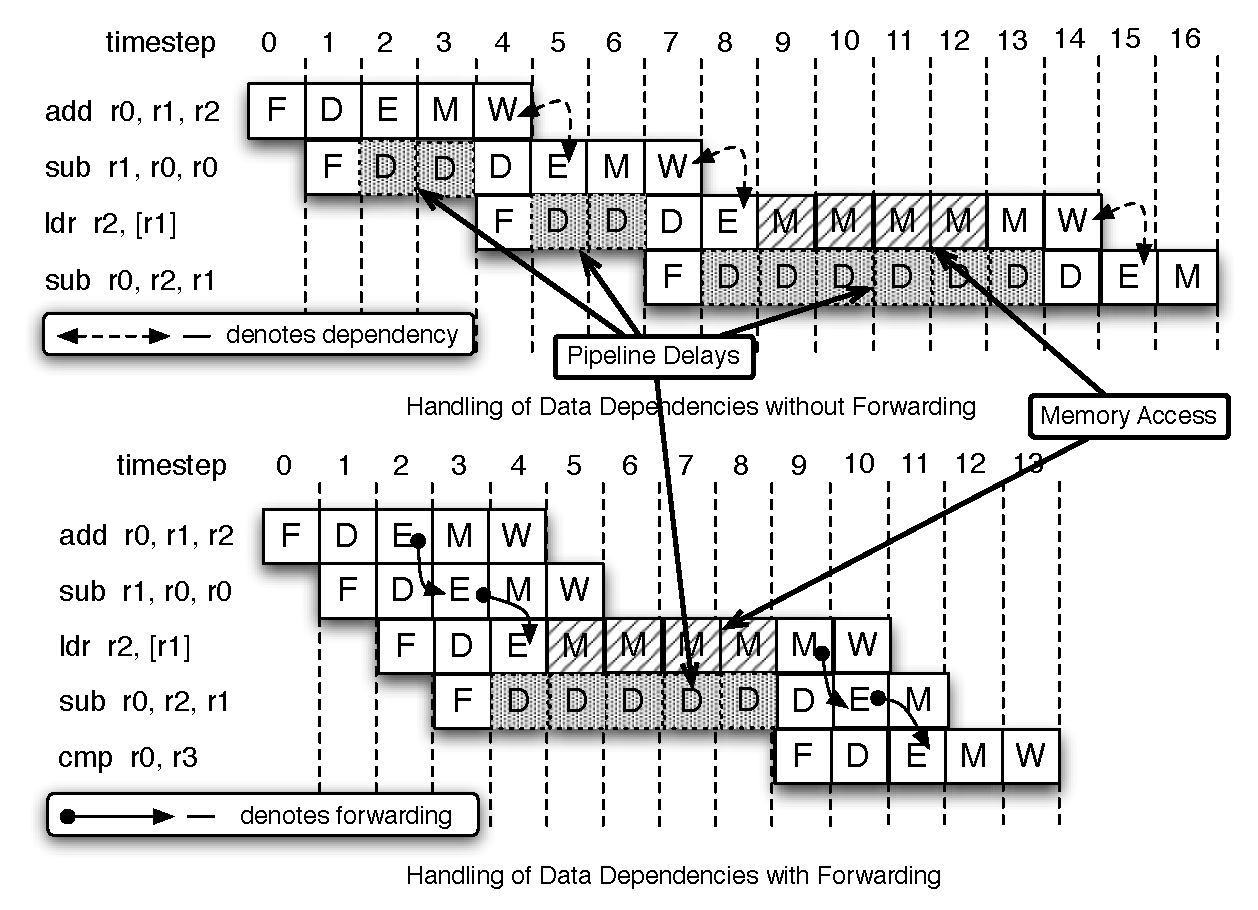
\includegraphics[scale=.6]{figs/data_depend_execution_non_interleaved}
\end{center}
\vspace{-10pt}
\caption{Handling of data dependencies in single threaded pipelines}
\label{fig:data_depend_execution_non_interleaved}
\end{figure}
No pipeline bubbles are needed for the first \emph{sub} instruction and \emph{ld} instruction because the data they depend on are forwarded with the forwarding paths.
However, the second \emph{sub} instruction after the \emph{ld} instruction still stalls. 
As mentioned earlier, forwarding relies on the results from the previous instruction being available before the previous instruction commits. 
In the case of longer latency operations, such as memory accesses, the data cannot be forwarded until it becomes available, so stalls are still required.
The memory access latency in the figure is arbitrarily chosen to be 5 cycles so the figure is not too long and instructions after the \emph{ld} instruction can be shown.  
We purposely leave out the details regarding memory accesses at this point, and will discuss it extensively in section~\ref{section:memory_system}.
We merely use the \emph{ld} instruction to illustrate the limitations of data forwarding.
They can address the data-dependencies caused by pipelining -- the read-after-write of register computations. 
However, they cannot address the data-dependencies caused by other long latency operations such as memory operations, so pipeline stalls are still needed.
More involved techniques such as the introduction of out-of-order execution or superscalar pipelines are used to mitigate the effects of long latency operations. 
We will discuss more of these in chapter~\ref{chapter:related} when we mention the related works.  

To understand the timing effects of handling data hazards, we discuss how to determine execution time for instructions using both methods of handling data hazards.  
With the simple method of inserting stalls, we need to know when the stalls will be inserted and how long the instruction will need to stall for.
This information can be determined by simply checking the previous instruction since stalls are inserted only if this instruction depends on the results of the previous instruction.
Within pipelines, the execution of most instructions are deterministic, so for the most part we can determine how long the stall will be by
checking the previous instruction.
Memory access instructions are an exception to instructions that have deterministic execution time, but as mentioned before, we will discuss these extensively in section~\ref{section:memory_system}.
For pipelines with data forwarding, we need to know in what situations the data forwarding circuitry cannot correctly forward the data to the next instruction.    
Although the pipeline dynamically forwards the data during run-time, the logic in the pipeline controller that enables and selects the correct forwarding bits only needs to keep track of a small set of previous instructions to detect data-dependencies.
The set of instructions it needs to check usually depends on the depth of the pipeline.  
Thus, static execution time analysis can detect forwarding by simply checking a short window of previous instructions to account for stalls accordingly. \todo{find papers to back this up}
We simplified greatly the execution time analysis discussed above to ignore effects from other pipeline mechanisms.
We wanted to simply focused on the effects of handling data-hazards through stalling or data-forwarding.  
We can see that both methods of handling data-hazards cause instruction execution time to depend previous instruction execution history. 
But the execution history that instruction execution time is dependent upon is small and temporary enough to be accounted for.
  
%The internal state of the branch predictor on the other hand is dependent on branch histories which may have happened arbitrarily long ago in the execution sequence,
%\todo{more complicated ways of handling data hazards include out-of-order execution\ldots}  

\begin{wrapfigure}{r}{0.5\textwidth}
  \vspace{-20pt}
  \begin{center}
    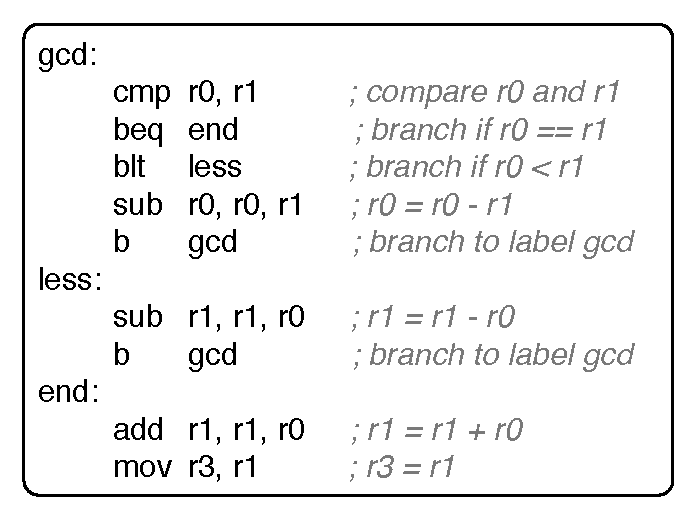
\includegraphics[scale=.65]{figs/sample_gcd_code}
  \end{center}
  \vspace{-20pt}
  \caption{Sample code for GCD with conditional branches}
  \label{fig:sample_gcd_code}
\end{wrapfigure}
Branches cause control-flow hazards in the pipeline; the instruction after the branch, which should be fetched the next cycle, is unknown until after the branch instruction is completed.
Conditional branches further complicates matters, as whether or not the branch is taken depends on an additional condition that could possible be unknown when the conditional branch is in execution. 
The code segment in figure~\ref{fig:sample_gcd_code} shows assembly instructions from the ARM instruction set architecture (ISA) that implement the Greatest Common Divisor (GCD) algorithm using conditional branch instructions \emph{beq} (branch equal) and \emph{blt} (branch less than).  
Conditional branch instructions in ARM branch based on conditional bits that are stored in a processor state register and set with special compare instructions\todo{cite arm manual}.
The \emph{cmp} instruction is one such compare instruction that subtracts two registers and sets the conditional bits according to the results.
The GCD implementation shown in the code uses this mechanism to determine whether to continue or end the algorithm.
Figure~\ref{fig:branch_execution_non_interleaved_pipeline} show two ways branches can be handled in a single-threaded pipeline. 

\begin{figure}
\begin{center}
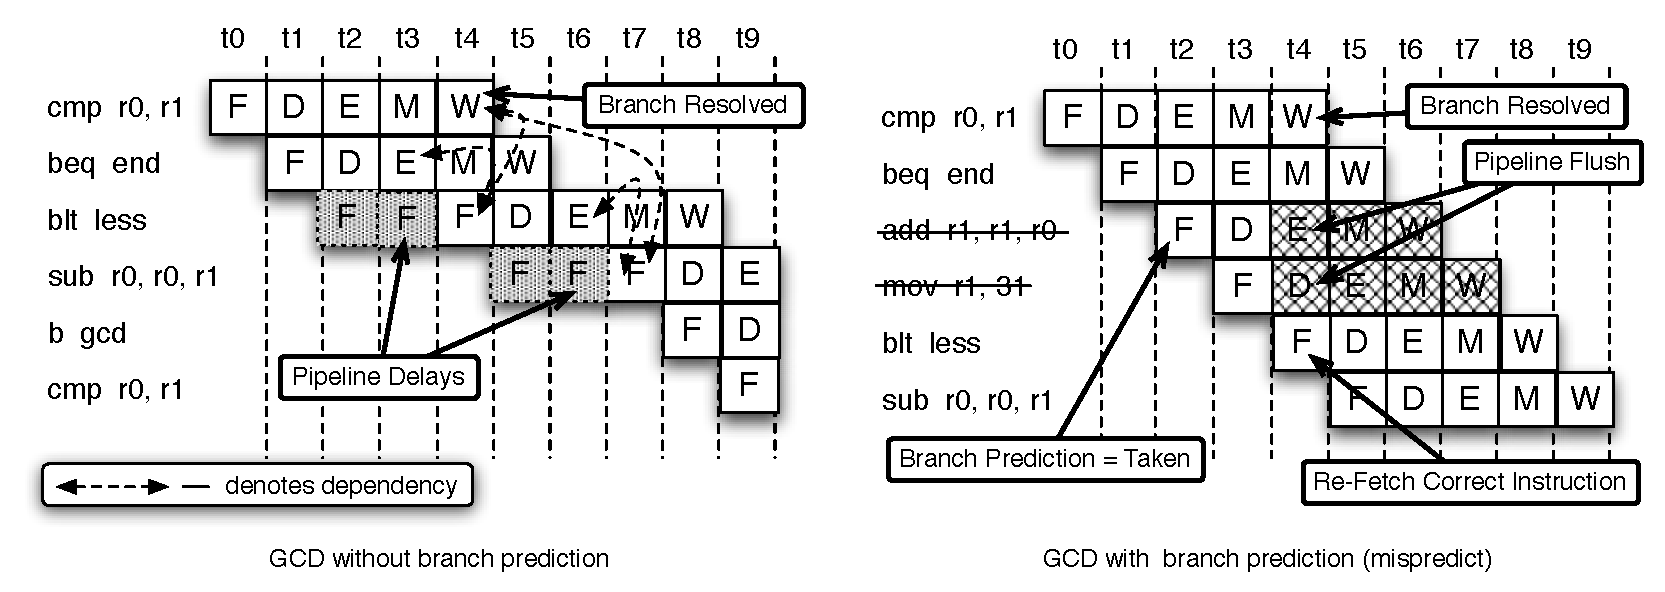
\includegraphics[scale=.58]{figs/branch_execution_non_interleaved_pipeline}
\end{center}
\vspace{-10pt}
\caption{Handling of conditional branches in single threaded pipelines}
\label{fig:branch_execution_non_interleaved_pipeline}
\end{figure}
Similar to handling data-hazards, a simple but effective way of handling control-flow hazards is by simply stalling the pipeline until the branch instruction completes.
This is shown on the left of figure~\ref{fig:branch_execution_non_interleaved_pipeline}. 
Two pipeline delays (or bubbles) are inserted after each branch instruction to wait until address calculation is completed.
The dependencies between instructions are also drawn out to make clear why the pipeline bubbles are necessary.
In order for the \emph{blt} instruction to be fetched, its address must be calculated during the execution stage of the \emph{beq} instruction.
At the same time, because \emph{beq} is a conditional branch, whether or not the branch is taken depends on the \emph{cmp} instruction.
The pipeline here is assumed to have forwarding circuitry, so the addresses calculated by the branch instructions and the results of the \emph{cmp} instruction can be used before the instructions are committed.
The performance penalty incurred is the pipeline delays inserted to wait for the branch address calculation to complete.
Conditional branches will also incur extra delays for deeper pipelines if the branch condition cannot be resolved in time. 
Some architectures enforce the compiler to insert one or more non-dependent instructions after a branch that is always executed before the change in control-flow of the program. 
These are called branch delay slots and can mitigate the branch penalty, but become less effective as pipelines grow deeper because the longer delay slots are required.  

In attempt to remove the need of inserting pipeline bubbles, branch predictors were invented to predict the results of a branch before it is resolved\todo{citation}.
%Branch predictors have been heavily researched.
Many clever branch predictors have been proposed, and they can accurately predict branches up to 93.5\%\todo{citation}.
%With branch predictor, the pipeline fetches the next instruction based upon the results of the branch prediction, and continues to execute speculatively.
Branch predictors predict the condition and target addresses of branches, so pipelines can speculatively continue execution based upon the prediction.  
If the prediction was correct, no penalty occurs for the branch, and execution simply continues. 
However, when a mispredict occurs, then the speculatively executed instructions need to be flushed and the correct instructions need to be refetched into the pipeline for execution.
The right of figure~\ref{fig:branch_execution_non_interleaved_pipeline} shows the execution of GCD in the case of a branch misprediction.
After the \emph{beq} instruction, the branch is predicted to be taken, and the \emph{add} and \emph{mov} instructions from the label \emph{end} is directly fetched into execution. 
When the \emph{cmp} instruction is completed, a misprediction is detected, so the \emph{add} and \emph{mov} instruction are flushed out of the pipeline while the correct instruction \emph{blt} is immediately re-fetched and execution continues.
The misprediction penalty is typically the number of stages between fetch and execute, as those cycles are wasted executing instructions from an incorrect execution path.
This penalty only occurs on a mispredict, thus branch prediction typically yields better average performance and is preferred for modern architectures.
%However, for more complex architectures with caches or other hardware states, the effects of incorrectly fetched instructions on the state of the processor less well-known and studied. 
Nonetheless, it is important to understand the effects of branch prediction on execution time. 

Typical branch predictors predict branches based upon the history of previous branches encountered.  
As each branch instruction is resolved, the internal state of the predictor, which stores the branch histories, is updated and used to predict the next branch.
This implicitly creates a dependency between branch instructions and their execution history, as the prediction is affected by its history.
In other words, the execution time of a branch instruction will depend on the branch results of previous branch instructions.
During static execution timing analysis, the state of the branch predictor is unknown because is it often infeasible to keep track of execution history so far back.   
There has been work on explicitly modeling branch predictors for execution time analysis\todo{citation}, but the results are \todo{the results of branch predictor modeling for execution time analysis}.
The analysis needs to conservatively account for the potential branch mispredict penalty for each branch, which leads to overestimated execution times.
To make matters worse, as architectures grow in complexity, more internal states exist in architectures that could be affected by the speculative execution. 
For example, cache lines could be evicted when speculatively executing instructions from a mispredicted path, changing the state of the cache.  
%When instructions from the correct execution path are re-fetched at branch resolution, a cache miss could be resulted from the change in cache because of the branch misprediction.    
This makes a tight static execution time analysis extremely difficult, if not impossible; explicitly modeling all hardware states and their effects together often lead to an infeasible explosion in state space. 
On the other hand, although the simple method of inserting pipeline bubbles for branches could lead to more branch penalties, the static timing analysis is precise and straight forward, as no prediction and speculative execution occur. 
The timing analysis simply adds the branch penalty to the instruction after a branch. 
Additional penalties from a conditional branch can be accounted for by simply checking for instructions that modify the conditional flag above the conditional branch.
We explicitly showed this simple method of handling branches to point out an important trade-off between speculative execution for better average performance and consistent stalling for better predictability.
Average-case performance can be improved by speculation at the cost of predictability and potentially prolonging the worst-case performance.  
The challenge remains to maintain predictability while improving worst-case performance, and how pipeline hazards are handled play an integral part of tackling this challenge.           

\subsection{Pipeline Multithreading}
 Multithreaded architectures were introduced to improve instruction throughput over instruction latency.
The architecture optimizes thread-level parallelism over instruction-level parallelism to improve performance.
Multiple hardware threads are introduced into the pipeline to fully utilize thread-level parallelism. 
When one hardware thread is stalled, another hardware thread can be fetched into the pipeline for execution to avoid stalling the whole pipeline. 
To lower the context switching overhead, the pipeline contains physically separate copies of hardware thread states, such as registers files and program counters etc, for each hardware thread.
\begin{figure}
\begin{center}
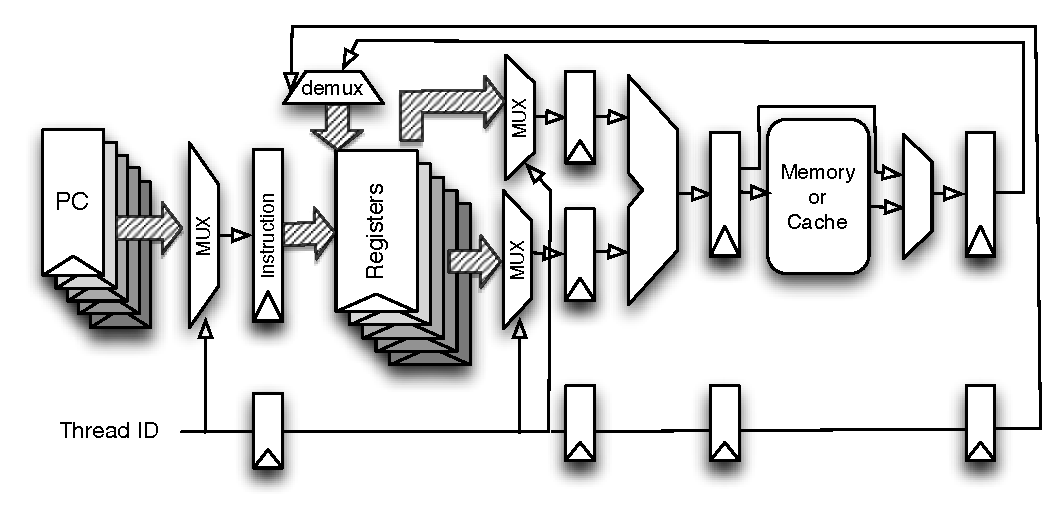
\includegraphics[scale=.8]{figs/multithreaded_pipeline_block}
\end{center}
\vspace{-30pt}
\caption{Simple Multithreaded Pipeline}
\label{fig:multi-thread pipeline simplified}
\end{figure}
Figure~\ref{fig:multi-thread pipeline simplified} shows a architectural level view of a simple multithreaded pipeline.
It contains 5 hardware threads, so it has 5 copies of the Program Counter (PC) and Register files.
Once a hardware thread is executing in the pipeline, its corresponding thread state can be selected by signaling the correct selection bits to the multiplexers.
The rest of the pipeline remains similar to a traditional 5 stage pipeline as introduced in Hennessy and Pattern\todo{citation}.   
The extra copies of the thread state and the multiplexers used to select them thus contribute to most of the hardware additions needed to implement hardware multithreading.

%The selection of threads for execution is one of the most important factors to fully utilize thread-level parallelism.
%If a thread is stalled waiting for memory access but gets selected to execute in the pipeline, then that instruction slot is wasted and the processor isn't fully utilized.
Ungerer et al.~\cite{Ungerer:2003:survey_multithreading} surveyed different multithreaded architectures and categorized them based upon the \todo{thread selection?} policy and the execution width of the pipeline.
The thread selection policy is the context switching scheme used to determine which threads are executing, and how often a context switch occurs.  
Coarse-grain policies manage hardware threads similar to the way operation systems manage software threads.
A hardware thread gain access to the pipeline and continues to execute until a context switch is triggered.
Context switches occur less frequently via this policy, so less hardware threads are required to fully utilize the processor.
Different coarse-grain policies trigger context switches with different events. 
Some trigger on dynamic events, such as cache miss or interrupts, and some trigger on static events, such as specialized instructions.
Fine-grain policies switch context much more frequently -- usually every processor cycle.
Both coarse-grain and fine-grain policies can also have different hardware thread scheduling algorithms that are implemented in a hardware thread scheduling controller to determine which hardware thread is switched into execution.  
The width of the pipeline refers to the number of instructions that can be fetched into execution in one cycle. 
For example, superscalar architectures have redundant functional units, such as multipliers and ALUs, and can dispatch multiple instructions into execution in a single cycle. 
Multithreaded architectures with pipeline widths of more than one, such as Sumultanous Multithreaded (SMT) architectures, can fetch and execute instructions from several hardware threads in the same cycle.

Multithreaded architectures typically bring additional challenges to execution time analysis of software running on them.
Any timing analysis for code running on a particular hardware thread needs to take into account not only the code itself, but also the thread selection policy of the architecture and sometimes even the execution context of code running on other hardware threads.
For example, if dynamic coarse-grain multithreading is used, then a context switch could occur at any point when a hardware thread is executing in the pipeline.
This not only has an effect on the control flow of execution, but also the state of any hardware that is shared, such as caches or branch predictors.    
Thus, it becomes nearly impossible to estimate execution time without knowing the exact execution state of other hardware threads and the state of the thread scheduling controller.
However, it is possible to for multithreaded architectures to fully utilize thread-level parallelism while still maintaining timing predictability.
Thread-interleaved pipelines use a fine-grain thread switching policy with round robin thread scheduling to achieve high instruction throughput while still allowing precise timing analysis for code running on its hardware threads. 
Below, its architecture and trade-offs are described and discussed in detail along with examples and explanation of how timing predictability is maintained.
Through the remainder of this chapter, we will use the term ``thread'' to refer to explicit hardware threads that have physically separate register files, program counters, and other thread states.
This is not to be confused the common notion of ``threads'', which is assumed to be software threads that is managed by operating systems with thread states stored in memory.

\subsection{Thread-Interleaved Pipelines}
\label{section:pret_thread_pipeline}
%\todo{Go through and make sure you don't say minimum threads as pipeline stages is a requirement, since later we have 4 threads in a give stage pipeine.}
\begin{figure}
  \vspace{-20pt}
  \begin{center}
    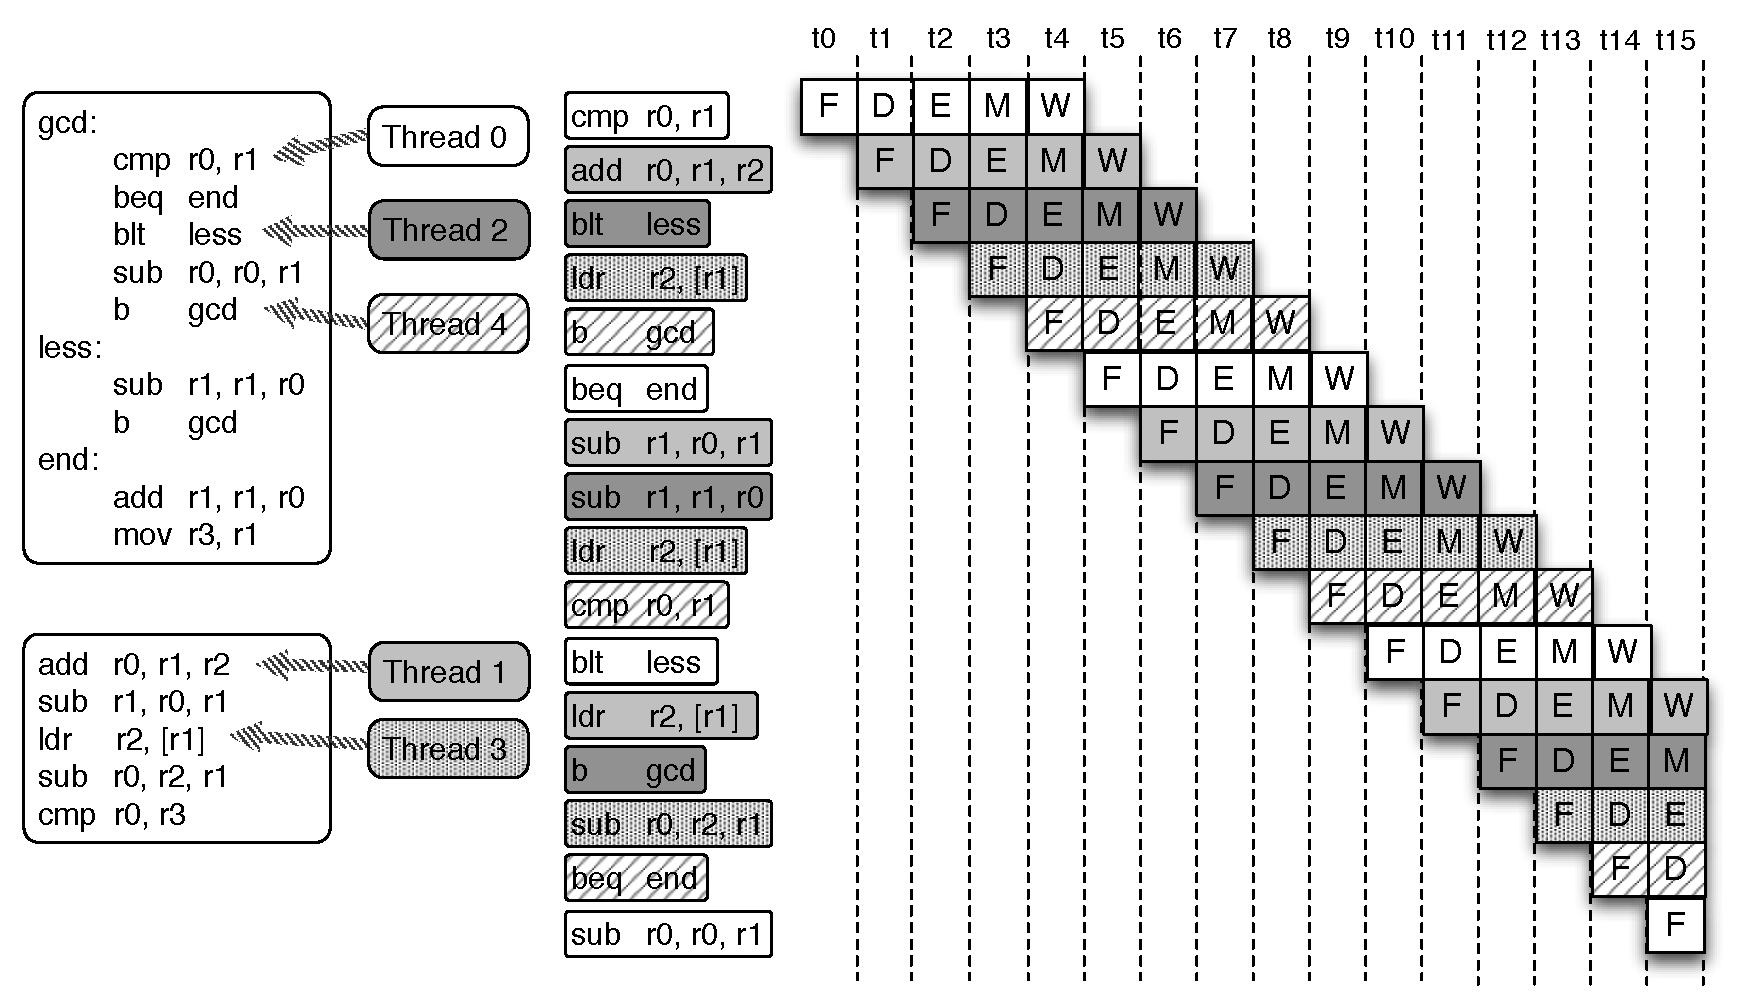
\includegraphics[scale=.55]{figs/thread-interleaved-execution}
  \end{center}
  \vspace{-20pt}
  \caption{Sample execution sequence of a thread-interleaved pipeline with 5 threads and 5 pipeline stages}
  \label{fig:execution_thread_interleaved_pipeline}
\end{figure}
The thread-interleaved pipeline was introduced to improve the response time of handling multiple I/O devices \todo{citation}.
I/O operations often stall from the communication with the I/O devices.
Thus, interacting with multiple I/O devices leads to wasted processor cycles that are idle waiting for the I/O device to respond.
By employing multiple hardware thread contexts, a hardware thread stalled from the I/O operations does not stall the whole pipeline, as other hardware threads can be fetched and executed.
% In a thread-interleaved pipeline, a thread context switch occurs every processor cycle, and the threads are cycled through in a round robin fashion. 
% This ensures each thread gets equal access to the process resource, so threads that aren't stalled are guaranteed to make progress.
Thread-interleaved pipelines use fine-grain multithreading; every cycle a context switch occurs and a different hardware thread is fetched into execution. 
The threads are scheduled in a deterministic round robin fashion. 
This also reduces the context switch overhead down to nearly zero, as no time is needed to determine which thread to fetch next.
Barely any hardware is required to implement round robin thread scheduling; a simple $log(n)$ bit up counter (for $n$ threads) would suffice.         
Figure~\ref{fig:execution_thread_interleaved_pipeline} shows an example execution sequence from a 5 stage thread-interleaved pipeline with 5 threads.
The thread-interleaved pipelines shown and presented in this thesis are all of single width.
The same code segments from figure~\ref{fig:sample_gcd_code} and figure~\ref{fig:sample_data_dependent_code} are being executed in this pipeline. 
Threads 0, 2 and 4 execute GCD (figure~\ref{fig:sample_gcd_code}) and threads 1 and 3 execute the data dependent code segment (figure~\ref{fig:sample_data_dependent_code}).
Each hardware thread executes as an independent context and their progress is shown in figure~\ref{fig:execution_thread_interleaved_pipeline} with thick arrows pointing to the execution location of each thread at t0.
We can observe from the figure that each time step an instruction from a different hardware thread is fetched into execution and the hardware threads are fetched in a round robin order.
At time step 4 we begin to visually see that each time step, each pipeline stage is occupied by a different hardware thread.
The fine-grained thread interleaving and the round robin scheduling combine to form this important property of thread-interleaved pipelines, which provides the basis for a timing predictable architecture design.

For thread-interleaved pipelines, if there are enough thread contexts, for example -- the same number of threads as there are pipeline stages, then at each time step no dependency exists between the pipeline stages since they are each executing on a different thread. 
As a result, data and control pipeline hazards, the results of dependencies between stages within the pipelines, no longer exist in the thread-interleaved pipeline.    
We've already shown from figure~\ref{fig:branch_execution_non_interleaved_pipeline} that when executing the GCD code segment on a single-threaded pipeline, control hazards stem from branch instructions because of the address calculation for the instruction after the branch.
However, in a thread-interleaved pipeline, the instruction after the branch from the same thread is not fetched into the pipeline until the branch instruction is committed.
Before that time, instructions from other threads are fetched so the pipeline is not stalled, but simply executing other thread contexts.
This can be seen in figure~\ref{fig:execution_thread_interleaved_pipeline} for thread 0, which is represented with instructions with white backgrounds.
The \emph{cmp} instructions, which determines whether next conditional branch \emph{beq} is taken or not, completes before the \emph{beq} is fetched at time step 5.
The \emph{blt} instruction from thread 0, fetched at time step 10, also causes no hazard because the \emph{beq} is completed before \emph{blt} is fetched.
The code in figure~\ref{fig:sample_data_dependent_code} is executed on thread 1 of the thread interleave pipeline in figure~\ref{fig:execution_thread_interleaved_pipeline}.
The pipeline stalls inserted from top of figure~\ref{fig:data_depend_execution_non_interleaved} are no longer needed even without a forwarding circuitry because the data-dependent instructions are fetched after the completion of its previous instruction.
In fact, no instruction in the pipeline is dependent on another because each pipeline stage is executing on a separate hardware thread context.
Therefore, the pipeline does not need to include any extra logic or hardware for handling data and control hazards in the pipeline. 
This gives thread-interleaved pipelines the advantage of a simpler pipeline design that requires less hardware logic, which in turns allows the pipeline clock speed to increase.
Thread-interleaved pipelines can be clocked at higher speeds since each pipeline stage contains significantly less logic needed to handle hazards.
The registers and processor states use much more compact memory cells compared to the logic and muxes used to select and handle hazards, so the size footprint of thread-interleaved pipelines are also typically smaller.

For operations that have long latencies, such as memory operations or floating point operations, thread-interleaved pipelines hides the latency with its execution of other threads. 
Thread 3 in figure~\ref{fig:execution_thread_interleaved_pipeline} shows the execution of a \emph{ld} instruction that takes the same 5 cycles as shown in figure~\ref{fig:data_depend_execution_non_interleaved}.
We again assume that this \emph{ld} instruction accesses data from the main memory. 
While the \emph{ld} instruction is waiting for memory access to complete, the thread-interleaved pipeline executes instructions from other threads.
The next instruction from thread 3 that is fetched into the pipeline is again the same \emph{ld} instruction.  
As memory completes its execution during the execution of instructions from other threads, we replay the same instruction to pick up the results from memory and write it into registers to complete the execution of the \emph{ld} instruction. 
It is possible to directly write the results back into the register file when the memory operation completes, without cycling the same instruction to pick up the results.
This would require hardware additions to support and manage multiple write-back paths in the pipeline, and a multi write ported register file, so contention can be avoided with the existing executing threads.
In our design we simply replay the instruction for write-backs to simplify design and piggy back on the existing write-back datapath.
%We showed a memory access instruction in our example, but the same reasoning is applied to floating point instructions or any long latency instruction.  
Multithreaded pipelines typically mark threads inactive when they are waiting for long latency operations.
Inactive threads are not fetched into the pipeline, since they cannot make progress even if they are scheduled. 
This allows the processor to maximize throughput by allowing other threads to utilize the idle processor cycles.   
However, doing so has non-trivial effects on thread-interleaved pipelines and the timing of other threads. 

First, if the number of ``active'' threads falls below the number of pipeline stages, then pipeline hazards are reintroduced; it is now possible for the pipeline to be executing two instructions from the same thread that depend on each other simultaneously. 
This can be circumvented by inserting pipeline bubbles when there aren't enough active threads. 
For example, as shown in figure~\ref{fig:three_thread_pipeline}, for our 5 stage thread-interleaved pipeline that has 5 threads, if two threads are waiting for main memory access and are marked inactive, then we insert 2 NOPs every round of the round-robin schedule to ensure that no two instructions from the same thread exists in the pipeline.
Note that if the 5 stage thread-interleaved pipeline contained 7 threads, then even if 2 threads are waiting for memory, no NOP insertion would be needed since instructions in each pipeline stage in one cycle would still be from a different thread.   
NOP insertions only need to occur when the number of active threads drops below the number of pipeline stages.   
\begin{figure}
  \vspace{-20pt}
  \begin{center}
    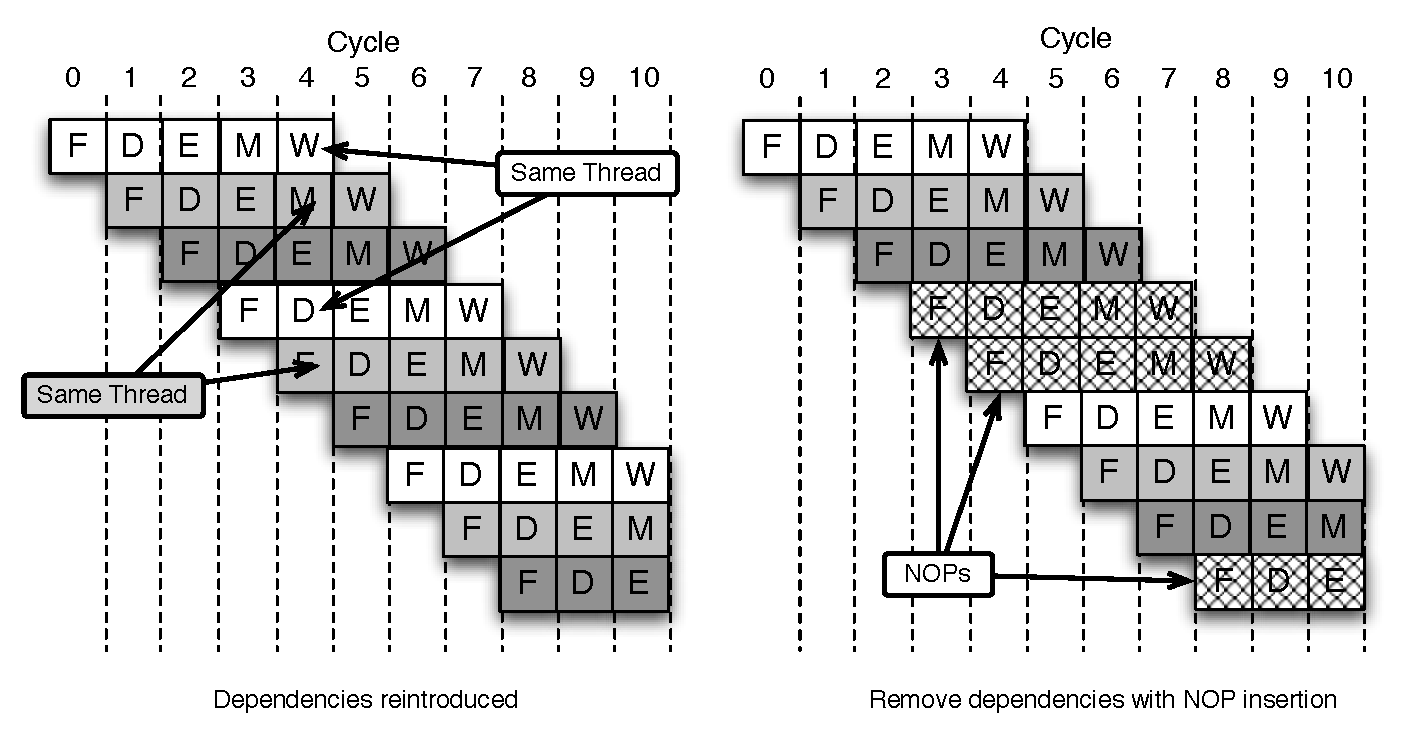
\includegraphics[scale=.6]{figs/three_thread_pipeline}
  \end{center}
  \vspace{-20pt}
  \caption{Execution of 5 threads thread-interleaved pipeline when 2 threads are inactive}
  \label{fig:three_thread_pipeline}
\end{figure}

The more problematic issue with setting threads inactive whenever long latency operations occur is the effect on the execution frequencies of other threads in the pipeline.
When threads are scheduled and unscheduled dynamically, the other threads in the pipeline would dynamically execute more or less frequently depending on how many threads are active.
This complicates timing analysis since the thread frequency of one thread now depends on the program state of all other threads. 
In order for multithreaded architectures to achieve predictable performance, \emph{temporal isolation} must exist in the hardware between the threads.
Temporal isolation is the isolation of timing behaviors of a thread from other thread contexts in the architecture.
With temporal isolation, the timing analysis is greatly simplified, as software running on individual threads can be analyzed separately without worry about the effects of integration. 
If temporal isolation is broken, any timing analysis needs to model and explore all possible combinations of program state of all threads, which is typically infeasible.
The round-robin thread scheduling of thread-interleaved pipelines is a way of achieving temporal isolation for a multithreaded architecture.
Unlike coarse-grain dynamically switched multithreaded architectures, thread-interleaved pipelines can maintain the same round-robin thread schedule despite the execution context of each thread within the pipeline. 
This is a step towards achieving temporal isolation amongst the threads, as the execution frequency of threads does not change dynamically.  
However, dynamically scheduling and unscheduling threads based upon long-latency operations breaks temporal isolation amongst threads.
Thus, our thread-interleaved pipeline does not mark threads inactive on long latency operations, but simply replays the instruction whenever the thread is fetched.  
Although this slightly reduces the utilization of the thread-interleaved pipeline, but threads are decoupled and timing analysis can be done individually for each thread without interference from other threads.
At the same time, we still preserve most of the benefits of latency hiding, as other threads are still executing during the long latency operation.

%TODO: exception handling
\todo{talk about xmos handling exceptions and our handling of exceptions here}

Shared hardware units within multithreaded architectures could also easily break temporal isolation amongst the threads. 
Two main issues arise when a hardware unit is shared between the threads. 
The first issue arises when shared hardware units share the same state between all threads. 
If the state of hardware unit is shared and can be modified by any thread, then it is nearly impossible to get a consistent view of the hardware state from a single thread during timing analysis.
Shared branch predictors and caches are prime examples of how a shared hardware state can cause timing inference between threads.
If a multithreaded architecture shares a branch predictor for all threads, then the branch table entries can be overwritten by branches from any thread.
This means that each thread's branches can cause a branch mispredict for any other thread. 
Caches are especially troublesome when shared between threads in a multithreaded architecture. 
Not only does it make the execution time analysis substantially more difficult, it also decreases overall performance for each thread due to cache thrashing, an event where threads continuously evict each other threads cache lines in the cache\todo{citation}.
To achieve temporal isolation between the threads, the hardware units in the architecture must not share state between the threads. 
Each thread must have its own consistent view of the hardware unit states, without the interference from other threads.
For example, each thread in our thread-interleaved pipeline contains its own private copy of the registers and thread states.    
We already showed why thread-interleaved pipelines do not need branch predictors because they remove control-hazards, and we will discuss a timing predictable memory hierarchy that uses scratchpads instead of caches in section~\ref{section:memory_system}.
The sharing of hardware state between threads also increases security risks in multithreaded architectures. 
Side-channel attacks on encryption algorithms\todo{cite} take advantage of the shared hardware states to disrupt and probe the execution time of threads running the encryption algorithm to crack the encryption key.
We will discuss this in detail in section~\ref{sec:app_side_channel_attack} and show how a predictable architecture can prevent timing side-channel attacks for encryption algorithms.   

The second issue that arises is that shared hardware units create structural hazards -- hazards that occur when a hardware unit needs to be used by two or more instructions at the same time.
Structural hazards typically occur in thread-interleaved pipelines when the shared units take longer than one cycle to access. 
The ALU, for example, is shared between the threads.
But because it takes only one cycle to access, there is no contention even when instructions continuously access the ALU in subsequent cycles.
On the other hand, a floating point hardware unit typically takes several cycles to complete its computation.
If two or more threads issue a floating point instruction in subsequent cycles, then contention arises, and the the second request must be queued up until the first request completes its floating point computation.   
This creates timing interference between the threads, because the execution time of a floating point instruction from a particular thread now depends on if other threads are also issuing floating point instructions simultaneously. 
If the hardware unit can be pipelined to accept inputs every processor cycle, then we can remove the the contention caused by the hardware unit, since accesses no longer need to be queued up.
The shared memory system in a thread-interleaved pipeline also creates structural-hazards in the pipeline.
In section~\ref{section:memory_system} we will discuss and present our memory hierarchy along with a redesigned DRAM memory controller that supports pipelined memory accesses.
%The assumption here is still that we have a single issue pipeline architecture.   
If pipelining cannot be achieved, then any timing analysis of that instruction must include a conservative estimation that accounts for thread access interference and contention management.
Several trade-offs need to be considered when deciding how to manage the thread contention to the hardware unit.

A time division multiplex access (TDMA) schedule to the hardware unit can be enforced to decouple the access time of threads remove timing interference.
A TDMA access scheme certainly creates an non-substantial overhead compared to conventional queuing schemes, especially if access to the hardware unit is rare and sparse.
However, in a TDMA scheme, each threads wait time to access the shared resource depends on the time offset in regards to the TDMA schedule, and is decoupled from the accesses of other threads.
Because of that, it is possible obtain a tighter worst case execution time analysis per thread.
For a TDMA scheme, the worst case access time occurs when an access just missed its time slot and must wait a full cycle before accessing the hardware unit.
For a conventional queuing scheme where each requester can only have one outstanding request, the worst case happens when every other requester has a request in queue, and the first request is just beginning to be serviced.   
At first, it may seem that the worst case execution time of a TDMA scheme may seem similar to the basic queuing scheme.
For timing analysis at an unknown state of the program, no assumption can be made on the TDMA schedule, thus the worst case time must be used for conservative estimations. 
However, because the TDMA access schedule is static, and access time is decoupled from other threads, there is potential to obtain tighter timing analysis for accesses by inferring access slot hits and misses for future accesses. 
For example, based upon the execution time offsets of a sequence of accesses to the shared resource, we may be able to conclude that at least one access will hit its TDMA access slot and get access right away.
We can also possibly derive more accurate wait times for the accesses that do not hit its access slots based upon the elapsed time between accesses.
An in depth study of WCET analysis of TDMA access schedules is beyond the scope of the thesis.
But these are possibilities now because there is no timing interference between the threads. 
A queue based mechanism would not be able to achieve better execution time analysis without taking into account the execution context of all other threads in the pipeline.

It is important to understand that we are not proclaiming that all dynamic behavior in systems are harmful. 
But only by achieving predictability in the hardware architecture can we begin to reason about more dynamic behavior in software.
For example, we discussed that dynamically scheduling threads in hardware causes timing interference. 
However, it is not the switching of threads that is unpredictable, but how the thread switching is triggered that makes it predictable.   
For example, the Giotto\todo{cite} programming model specifies a periodic software execution model that can contain multiple program states. 
If such a programming model was implemented on a thread-interleaved pipeline, different program states might map different tasks to threads or have different number of threads executing within the pipeline.
But by explicitly controller the thread switches in software, the execution time variances introduced is transparent at the software level, allowing potential for timing analysis.

%TODO: Talk about the trade-offs of threaded interleaved pipelines to summarize 
In this section we introduced a predictable thread-interleaved pipeline design that provides temporal isolation for all threads in the architecture.
The thread-interleaved pipeline favors throughput over single thread latency, as multiple threads are executed on the pipeline in a round robin fashion.  
We will present in detail our implementation of this thread-interleaved pipeline in chapter~\ref{chapter:ptarm}, and show how the design decisions discussed in this chapter are applied.

\section{Memory System}
\label{section:memory_system}
While pipelines designs continue to improve, memory technology has been struggling to keep up with the increase in clock speed and performance.
Even though memory bandwidth can be improved with more bank parallelization, the memory latency remains the bottleneck to improved memory performance.
Common memory technologies used in embedded systems contain a significant tradeoff between access latency and capacity. 
Static Random-Access Memories (SRAM) provide a shorter latency that allows single cycle memory access from the pipeline.
However, the hardware cost to implement each memory cell prevents SRAM blocks from being implemented with high capacity.
On the other hand, Dynamic Random-Access Memories (DRAM) use a more compact memory cell design that can easily be combined into larger capacity memory blocks.
But the memory cell of DRAMs must be constantly refreshed due to charge leakage, and the large capacity memory blocks often prohibit faster access latencies.
%TODO: talk about about embedded systems seldom need disk?
To bridge the latency gap between the pipeline and memory, smaller memories are placed in between the pipeline and larger memories to act as a buffer, forming a memory hierarchy.
The smaller memories give faster access latencies at the cost of lower capacity, while larger memories make up for that with larger capacity but slower access latencies. 
The goal is to speed up program performance by placing commonly accessed values closer to the pipeline and placing less accessed values farther away.

\subsection{Memory Hierarchy}
\subsubsection{Caches}
\begin{wrapfigure}{r}{0.5\textwidth}
  \vspace{-20pt}
  \begin{center}
    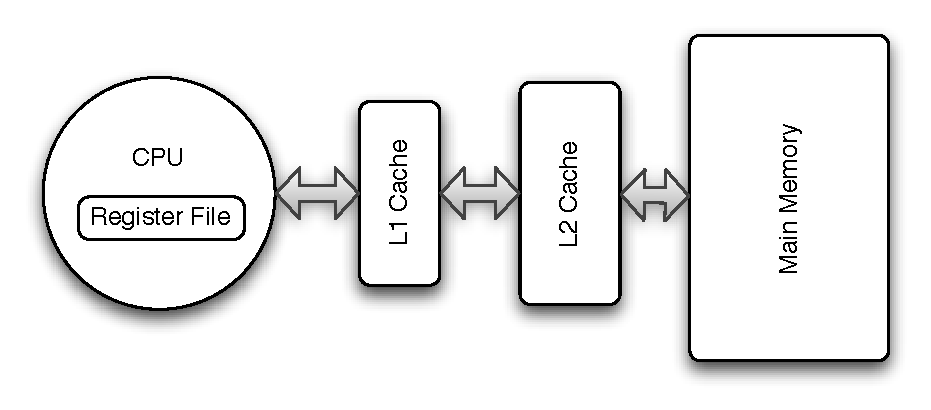
\includegraphics[scale=.5]{figs/conventional_mem_hierarchy}
  \end{center}
  \vspace{-20pt}
  \caption{Memory Hierarchy w/ Caches}
  \label{fig:conventional_mem_hierarchy}
  \vspace{-10pt}
\end{wrapfigure}   
A \emph{CPU Cache} (or cache) is commonly used in the memory hierarchy to manage the smaller fast access memory made of SRAMs.
The cache manages the contents of the fast access memory in hardware by leveraging the spatial and temporal locality of data accesses. 
The main benefits of the cache is that it abstracts away the memory hierarchy from the programmer.
When a cache is used, all memory accesses are routed through the cache. 
If the data from the memory access is in the cache, then a cache hit occurs, and the data is returned right away.
However, if data is not in the cache, then a cache miss occurs, and the cache controller fetches the data from the larger memory and adjusts the memory contents in the cache. 
The replacement policy of the cache is used to determine which cache line, the unit of memory replacement on caches, to replace. 
A variety of cache replacement policies have been researched and used to optimize for different memory access patterns of applications. 
In fact, modern memory hierarchies often contain multiple layers of hierarchy to balance the tradeoff between speed and capacity.
A commonly used memory hierarchy is shown in figure~\ref{fig:conventional_mem_hierarchy}.
If the data value is not found in the L1 cache, then it is searched for in the L2 cache. 
If the L2 cache also misses, then the data is retrieved from main memory, and sent back to the CPU while the L1 and L2 cache update its contents.
Different replacement policies can be used at different levels of the memory hierarchy to optimize the hit rate or miss latency of the memory access.

When caches are used, the program is oblivious to the different levels of memory hierarchy because they are abstracted away from the program; the cache gives its best-effort to optimize memory access latencies.
Whether or not an access hits the cache or goes all the way out to main memory is hidden from the program.
Thus, the programmer does not need to put in any effort, and can get a reasonable amount of performance. 
Furthermore, when programs are ported to another architecture with a different cache configuration, no change in the program is required to still obtain a reasonable amount of performance from the hardware.   
For general purpose applications, this gives the ability to improve design time and decrease design effort, which explains the cache's popularity. 

However, the cache makes no guarantees on actual memory access latencies and program performance. 
The execution time of programs could highly vary depending on a number different factors -- cold starts, previous execution contexts, interrupt routines, and even branch mispredictions that cause unnecessary cache line replacements.  
Thus, when execution time is important, the variability and uncontrollability of caches may outweigh the benefits they provide. 

The cache's internal states include the controller state and memory contents. 
As the programmer cannot explicitly control the state of the cache, it is extremely difficult to analyze execution time on systems with caches.
At an arbitrary point of execution, if the state of the cache is unknown, a conservative worst-case execution time analysis needs to assume the worst case, as if the memory access went directly to main memory.
In order to acquire tighter execution time analysis, the cache must be modeled with program execution to predict the cache state.
The ease of such modeling depends on the replacement policy used in the cache.

For example, the \emph{Least Recent Used} (LRU) replacement policy replaces the least recently used cache line whenever an eviction occurs. 
Within a basic block, a code segment without a control flow change, the contents of a cache with $N$ cache lines can be fully known after $N$ different memory accesses~\cite{Heckmann2003processor}.  
The $N$ different memory accesses will evict all cache lines in the cache prior to the basic block, and fill them with the memory contents of the $N$ accesses. 
In this case, the analysis assumes $N$ initial cache misses before the cache state is known.
However, the cache state is destroyed when analysis hits a control flow merge with another path.
Thus, the usefulness of this analysis depends on $N$ and how long basic blocks are in programs.  
In practice, the complexity of modern programs and memory architectures often introduce a high variability in program execution time, rendering analysis imprecise. 

Even outside of the context of real-time applications, caches can present unintended side effects.
For applications that require extreme high speed, the best-effort memory management that caches offer simply is not good enough.
Programs often need to be tuned and tailored to specific cache architectures and parameters to achieve the desired performance. 
In order to tune algorithm performance, algorithm designers are required to understand the abstracted away memory architecture and enforce data access patterns that conform to the cache size and replacement policy.   
For example, instead of operating on entire rows or columns of an array, algorithms are rewritten to operate on a subset of the data at a time, or blocks, so the faster memory in the hierarchy can be reused.
This technique is called \emph{Blocking}~\cite{Lam91thecache}, and is very well-known and commonly used.   
%\todo{talk about LAPACK? Libraries that tune programs to caching}.
%In this case, we see that the hidden memory hierarchy actually could degrade program performance.    

Multithreaded threaded architectures with shared caches among the hardware threads can suffer from \emph{cache thrashing}, an effect where different threads' memory accesses evict the cached lines of others.
With multiple hardware threads, it is extremely difficult for threads have any knowledge on the state of the cache, because it is simultaneously being modified by other threads in the system. 
As a result, the hardware threads have no control over which level in the memory hierarchy they are accessing, and the performance highly varies depending on what is running on other hardware threads. 

For multicore architectures, caches create a data coherency problem when data needs to be consistent between the multiple cores.
When the multiple cores are sharing memory, each core's private cache may cache the same memory address. 
If one core writes to a memory location that is cached in its private cache, then the other core's cache would contain stale data. 
Various methods such as bus snooping or implementing a directory protocol~\cite{Stenstrom:1990:SCC:79809.79810} have been proposed to keep the data consistent in all caches. 
Implementing a scalable and efficient cache coherence scheme is still a hot topic of research today.

\subsubsection{Scratchpads}
We cannot argue against the need for a memory hierarchy, as there is an undeniable gap between processor and DRAM latency.
However, instead of abstracting away the memory hierarchy, we propose to \emph{expose} the memory layout to the software.  

\emph{Scratchpads} were initially proposed for their power saving benefits over caches~\cite{Banakar2002}.
Scratchpads can be found in the Cell processor~\cite{cellproc}, which is used in Sony PlayStation 3 consoles, and NVIDIA's 8800 GPU, which provides 16KB of SPM per thread-bundle~\cite{8800gpu}.
Scratchpads use the same memory technology (SRAMs) as caches, but do not implement the hardware controller to manage their memory contents.
%Without the hardware controller, scratchpads do not manage its memory contents in hardware.
Instead, scratchpads occupy a distinct address space in memory when they are used as fast access memory.
Memory accesses that access the specific scratchpad address space will go to the scratchpad, and other accesses will go to main memory. 
Because in hardware scratchpads do not need to check whether the data is on the scratchpad or not, they have a reduced access latency, area and power consumption compared to caches~\cite{Banakar2002}. 

\begin{wrapfigure}{r}{0.45\textwidth}
  \vspace{-20pt}
  \begin{center}
    \includegraphics[scale=.5]{figs/pret_mem_hierarchy}
  \end{center}
  \vspace{-10pt}
  \caption{Memory Hierarchy w/ Scratchpads}
  \label{fig:pret_mem_hierarchy}
\end{wrapfigure}   

Unlike caches, which overlay their address space with main memory to hide the hierarchy, scratchpads explicitly \emph{expose} the memory hierarchy, as figure~\ref{fig:pret_mem_hierarchy} illustrates.  
The exposed memory hierarchy gives software full control over the management of memory contents in the hierarchy.
Data allocated on the scratchpad will have single cycle access latencies, while other data will take the full DRAM access latency. 
The memory access latency for each request now depends only on the access address, and not that state of another hardware controller. 
This drastically improves the predictability of memory access times, and removes the variability of execution time introduced with caches.
However, this places the burden of memory management on the programmer or compiler toolchains.  
The Cell processor~\cite{cellproc} is often criticized for being difficult to program, and one of the main reason is its use of scratchpads. 
Programmers have become accustomed to a uniform memory space, making it difficult to adjust to the non uniform memory space that must be explicitly managed.

Embedded system designs inherently need to deal with limited resources and other design constraints, such as limited memory or hard timing deadlines.    
Thus, the design of such systems often requires analysis of memory usage and latency to ensure that the constraints are met.
These analysis results can be used to generate automatic allocation schemes for scratchpads, lessening the burden on programmers.
Two allocation schemes are commonly employed to manage the contents of scratchpads in software.
\emph{Static allocation schemes} allocate data on the scratchpad during compile time, and the contents allocated on the scratchpad do not change throughout program execution. 
Static scratchpad allocation schemes~\cite{Suhendra2005WCETSPM, Patel2008PRETSPM} often use heuristics or a compiler-based static analysis of the program to find the most commonly executed instructions or data structures.
These are allocated statically on the scratchpad to improve program performance. 
\emph{Dynamic allocation schemes} modify the data on the scratchpad during run time in software through DMA mechanisms.
The allocation could either be automatically generated and inserted by the compiler, or explicitly specified by the user programmatically.
Higher level models of computation, such as Synchronous Dataflow (SDF)~\cite{lee_sdf} or Giotto~\cite{henzinger_giotto}, expose more structure and semantics of the model for better analysis, which can be used to optimize scratchpad allocation dynamically.
Bandyopadhyay~\cite{Bandyopadhyay06_AutomatedMemoryAllocationOfActorCodeDataBufferInHeterochronous} presents an automated memory allocation of scratchpads for the execution of Heterochronous Dataflow models.
The Heterochronous Dataflow (HDF) model is an extension to the Synchronous Dataflow (SDF) model with finite state machines (FCM). 
The HDF models contain different program states.
Each state executes a SDF model that contains actors communicating with each other. 
Bandyopadhyay analyzes the actor code and the data that is communicated in each HDF state, and derives an optimized scratchpad allocation for each state. 
The scratchpad allocation code is automatically inserted into the code to dynamically change the scratchpad contents during state transitions, so the memory allocation is optimized for the execution of each HDF state. 
This allocation not only shows roughly a 17\% performance improvement compared to executions using LRU caches, but also a more predictable program performance.

The underlying memory technology that is used to make both scratchpads and caches is not inherently unpredictable, as SRAMs provide constant low-latency access time. 
%However, caches manage the contents of the SRAM in hardware. 
However, by using caches in the memory hierarchy, the hierarchy is hidden from the programmer, and the hardware managed memory contents create highly variable execution times with unpredictable access latencies. 
Scratchpads on the other hand expose the memory hierarchy to the programmer, allowing for more predictable and repeatable memory access performances.
Although the allocation of scratchpads requires more programming effort, it also provides opportunity for high efficiency, as it can be tailored to specific applications.   
Thus, in our time-predictable architecture, scratchpads are employed as our fast-access memory. 

\subsection{DRAM Memory Controller}
Because of its high capacity, DRAMs are often employed in modern embedded systems to cope with the increasing code and data sizes.  
However, bank conflicts and refreshes within the DRAM can cause memory accesses to stall, further increasing the memory latency. 
Modern memory controllers are designed to optimize average-case performance by queueing and reordering memory requests to improve the throughput of memory requests. 
This results in unpredictable and varying access times along with an increased worst-case access time for each memory request.
In this section we will present a DRAM memory controller that privatizes DRAM banks with scheduled memory refreshes to provide improved worst-case latency and predictable access times.    
The contributions from this section are research done jointly with the several co-authors from Reineke et. al~\cite{ReinekeLiuPatelKimLee11_PRETDRAMControllerBankPrivatizationForPredictability}. 
We do not claim sole credit for this work, and the summary is included in this thesis only for completeness. 
We will first give some basic background on DRAM memories, then present the predictable DRAM controller designed.

\subsubsection{DRAM Basics}

\begin{figure}[h]
\begin{center}
\vspace{-8mm}
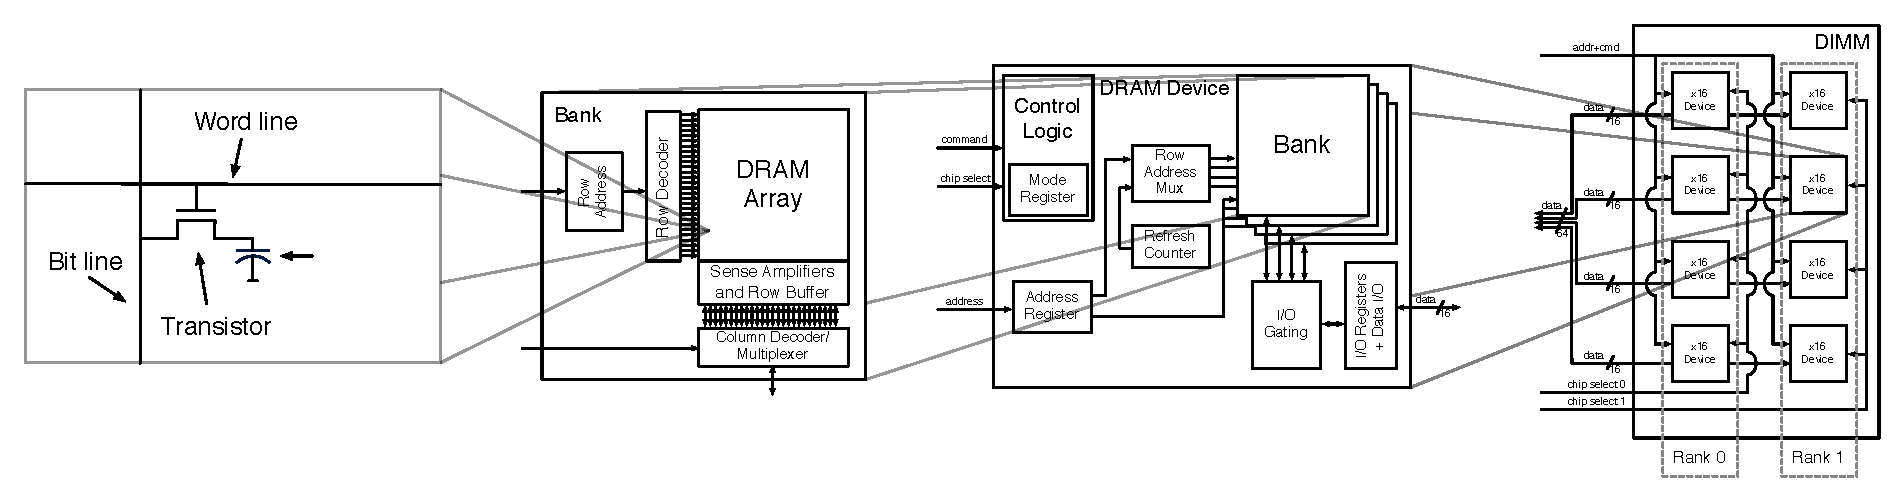
\includegraphics[width=\textwidth]{figs/dram-overview.pdf}
\vspace{-8mm}
\caption{A dual-ranked dual in-line memory module.}\label{fig:dram_basics}
\vspace{-5mm}
\end{center}
\end{figure} 

Figure~\ref{fig:dram_basics} shows the structure of a dual ranked in-line DDRII DRAM module.
Starting from the left, a basic \textbf{\emph{DRAM cell}} consists of a capacitor and a transistor. 
The capacitor charge determines the value of the bit, which can be accessed by triggering the transistor. 
Because the capacitor leaks charge, it must be refreshed periodically, typically every 64 ms or less~\cite{jedec}.

A \textbf{\emph{DRAM array}} is made of a two-dimensional array of DRAM cells.
Each access made to the DRAM array goes through two phases: a row access followed by one or more column accesses.   
During the row access, one of the rows in the DRAM array is moved into the row buffer.
To read the value in the row buffer, the capacitance of the DRAM cells is compared to the wires connecting them with the row buffer.
The wires need to be precharged close to the voltage threshold so the sense amplifiers can detect the bit value.
Columns can be read and written to quickly after the row is in the row buffer. 

The \textbf{\emph{DRAM device}} consists of banks formed of DRAM arrays. 
Modern DRAM devices have multiple banks, control logic, and I/O mechanisms to read from and write to the data bus, as shown in the center of figure \ref{fig:dram_basics}.
Banks can be accessed concurrently, but the data, command and address busses, which is what the memory controller uses to send commands to the DRAM device, are shared within the device. 
The following table\footnotemark\ lists the four most important commands and their function:
\footnotetext{This table is as shown in ~\cite{ReinekeLiuPatelKimLee11_PRETDRAMControllerBankPrivatizationForPredictability}}
%\begin{table}
\begin{center}
\begin{smalltabular}{p{13mm}p{6mm}p{10cm}}
Command 				& Abbr. & Description\\\hline
Precharge    			& PRE   & Stores back the contents of the row buffer into the DRAM array, and prepares the sense amplifiers for the next row access.\\
Row\hspace{13mm} access & RAS	& Moves a row from the DRAM array through the sense amplifiers into the row buffer.\\
Column access 			& CAS   & Overwrites a column in the row buffer or reads a column from the row buffer.\\
Refresh					& REF	& Refreshes several\footnotemark\ rows of the DRAM array. This uses the internal refresh counter to determine which rows to refresh.\\
\end{smalltabular}
%\caption{Overview of DDR2 Commands~\cite{ReinekeLiuPatelKimLee11_PRETDRAMControllerBankPrivatizationForPredictability}}
\label{tab:ddr2-commands}
\end{center}
%\end{table}
\footnotetext{The number of rows depends on the capacity of the device.}

To perform reads or writes, the controller first sends the PRE command to precharge the bank containing the data. 
Then, a RAS is issued to select the row, and one or more CAS commands can be used to access the columns within the row. 
Accessing columns from the same row does not require additional PRE and RAS commands, thus higher throughput can be achieved by performing column accesses in burst lengths of four to eight words.  
Column accesses can immediately be followed by a PRE command to decrease latency when accessing different rows. 
This is known as auto-precharge (or closed-page policy).
Refreshing of the cells can be done in two ways.
One common way is to issue a refresh command that refreshes all banks of the device simultaneously. 
The refresh latency depends on the capacity of the device, but the DRAM device manages a counter to step through all the rows.
The rows on the device could also be manually refreshed by performing row accesses to them.
Thus, the memory controller could perform row accesses on every row within the 64 ms refresh period.
This requires the memory controller to keep track of the refresh status of the device and issue more refresh commands, but each refresh takes less time because it is only a row access. 

\textbf{\emph{DRAM modules}} are made of several DRAM devices integrated together for higher bandwidth and capacity. 
A high-level view of the dual-ranked dual in-line memory module (DIMM) is shown in the right side of figure~\ref{fig:dram_basics}.
The DIMM has eight DRAM devices that are organized in two ranks.
The two ranks share the address, command inputs, and the 64-bit data bus.
The chip select is used to determine which ranks are addressed.
All devices within a rank are accessed simultaneously when the rank is addressed, and the results are combined to form the request response.  
% Due to the sharing of I/O mechanisms within a device, consecutive accesses to the same rank are more constrained than consecutive accesses to different ranks, which only share the command and address as well as the data bus.
% We later exploit this subtle difference by restricting consecutive accesses to different ranks to achieve more predictable access latencies.  
% We explain this in more detail in \ref{sec:pret_dram_controller}. 

Our controller makes use of a feature from the DDR2 standard known as posted-CAS.  
Unlike DDR or other previous versions of DRAMs, DDR2 can delay the execution of CAS commands (posted-CAS) for a user-defined latency, known as the additive latency ($AL$). 
Posted-CAS can be used to resolve command bus contention by sending the posted-CAS earlier than the corresponding CAS needs to be executed.

Table~\ref{table:ddr2-constraints} gives an overview of timing parameters for a DDR2-400 memory module.
These timing constraints come from the internal structure of DRAM modules and DRAM cells.
For example, $t_{RCD}, t_{RP}$, and $t_{RFC}$ are from the structure of DRAM banks that are accessed through sense amplifiers that need to be precharged.
$t_{CL}, t_{WR}, t_{WTR}$, and $t_{WL}$ result from the structure of DRAM banks and DRAM devices.
The four-bank activation window constraint $t_{FAW}$ constrains rapid activation of multiple banks that would result in too high of a current draw.
The memory controller must conform to these timing constraints when sending commands to the DDR2 module.  
%The additive latency, $t_{AL}$, can be set by the user and determines how many cycles after a posted-CAS a CAS is executed.
Here we only give a quick overview of DRAMs, we refer more interested readers to Jacob et al.~\cite{JaNgWa07} for more details.

\begin{table}[h]
\begin{center}
\begin{smalltabular}{l p{2.0cm} p{10cm}}
Parameter	& Value \footnotemark & Description \\\hline
$t_{RCD}$			& 3						& \textbf{Row-to-Column delay}: time from row activation to first read or write to a column within that row.\\
$t_{CL}$			& 3						& \textbf{Column latency}: time between a column access command and the start of data being returned.\\
$t_{WL}$			& $t_{CL}-1=2$			& \textbf{Write latency}: time after write command until first data is available on the bus.\\
$t_{WR}$			& 3						& \textbf{Write recovery time}: time between the end of a write data burst and the start of a precharge command.\\
%$t_{CCD}$			& $\burstlength/2$ 				& CAS to CAS command delay. Minimum time between two read commands or two write commands.\\
$t_{WTR}$ 			& 2 					& \textbf{Write to read time}: time between the end of a write data burst and the start of a column-read command.\\% Allows the sense amplifiers to restore the data in the DRAM array.\\
$t_{RP}$			& 3						& \textbf{Row precharge time:} time to precharge the DRAM array before next row activation.  \\
%$t_{RTRS}$			& 1\todo{check this}	& Rank-to-rank switching time.\\ 
$t_{RFC}$			& 21					& \textbf{Refresh cycle time}: time interval between a refresh command and a row activation.\\
%$t_{REFI}$			& 1560    				& Refresh to refresh interval \\
%$t_{RAS}$ 			& $t_{RCD}+t_{WL}+t_{WR} = 8$ & Minimum time after an activate command to a bank until that bank is allowed to be precharged.\\
%$t_{RC}$			& $t_{RAS}+t_{RP}=11$	& Row cycle time: minimum time between successive activate commands to the same bank.\\
%$t_{RTP}$			&   			& Minimum time between a precharge command on a bank and a successive activate command.\\
$t_{FAW}$			& 10					& \textbf{Four-bank activation window}: interval in which maximally four banks may be activated.\\
$t_{AL}$			& set by user			& \textbf{Additive latency}: determines how long posted column accesses are delayed.
\end{smalltabular}
%\todo{group constraints by their origin: constraints due to DRAM array structure, constraints due to sharing within DRAM device, constraints due to sharing of bus among ranks}
\end{center}
\caption{Overview of DDR2-400 timing parameters of the Qimonda HYS64T64020EM-2.5-B2.~\cite{ReinekeLiuPatelKimLee11_PRETDRAMControllerBankPrivatizationForPredictability}}\label{table:ddr2-constraints}
\end{table}
\footnotetext{In cycles at 200 MHz}

\subsubsection{Predictable DRAM Controller}
\label{sec:pret_dram_controller}
We will split the discussion of the predictable DRAM controller into its backend and frontend. 
The backend translates memory requests into DRAM commands that are sent to the DRAM module.
The frontend manages the interface to the pipeline along with the responsibility of scheduling refreshes.
Here we specifically refer to a DDR2 667MHz/PC2-5300 memory module operating at 200Mhz, which has a total size of 512MB over two ranks with four banks on each rank.
While our discussion of the design of this DRAM controller is specific to our DDR2 memory module, the key design features are applicable to other modern memory modules.

\paragraph{Backend}
Conventional DRAM memory controllers view the entire memory device as one resource, and any memory request can access the whole DRAM device. 
Subsequent memory accesses can target the same bank within the DRAM, which results in the need for memory requests to be queued and serviced sequentially, without exploiting bank parallelism.
Our controller views the memory devices as independent resources partitioned by banks. 
Specifically, we partition our memory module into four \emph{resources}, each consisting of two banks within the same rank. 
The banks within each resource can be arbitrarily chosen, but all banks within a resource must belong to the same rank, and each of the ranks must contain at least two resources.
This is to avert access patterns that would incur high latency from the contention for the shared busses within banks and ranks.
The partitioning of the memory device allows us to fully exploit bank parallelism by accessing the resources in a periodic and pipelined fashion.
The periodic access scheme to the four resources interleaves each memory access between the ranks.
Subsequent accesses to the same rank go to the other resource, grouped from banks.  
Figure~\ref{fig:backend} shows an example of the following access requests: read from resource 0 in rank 0, write to resource 1 in rank 1, and read from resource 2 in rank 0. 

\begin{figure}[h]
\begin{center}
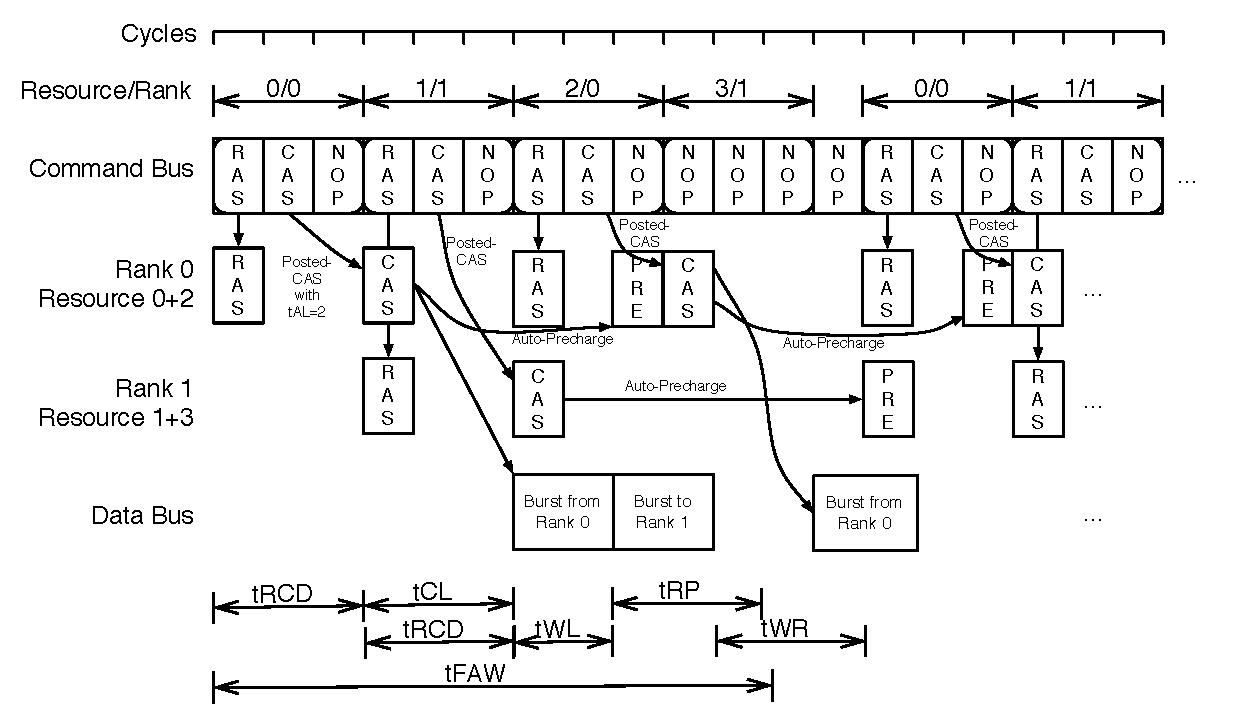
\includegraphics[width=0.92\linewidth]{figs/backend}
\end{center} 
\caption{The periodic and pipelined access scheme employed by the backend~\cite{ReinekeLiuPatelKimLee11_PRETDRAMControllerBankPrivatizationForPredictability}.}
\label{fig:backend}
\end{figure}

Each access request is translated into a RAS (Row Access), posted-CAS (Column Access) and NOP command. 
An access slot is formed of all three commands.  
The NOP command in the access slot is inserted between any two consecutive requests to avoid a collision on the data bus that occurs when a read request follows and a write request.
This collision is cause by the one cycle offset between the read and write latencies. 
The RAS command moves a row into the row buffer, and the CAS command accesses the columns within the row loaded into the row buffer. 
CAS commands can be either reads or writes, causing a burst transfer of $8 \cdot 4 = 32$ bytes that occupies the data bus for two cycles (as two transfers occur in every cycle).
We send a posted-CAS instead of a normal CAS in order to meet the row to column latency shown in table~\ref{table:ddr2-constraints}.
This latency specifies that the RAS command and the first CAS command need to be 3 cycles apart.  
However, manually issuing a CAS command to the first resource 3 cycles after its RAS command would cause a command bus conflict with the RAS command for the second resource.
Thus, we instead set the additive latency $t_{AL}$ to 2 and use the posted-CAS that offsets the CAS command to conform to the row to column latency.
This allows our memory controller to preserve our pipelined access scheme while meeting the latency requirements of the DRAM.   
We use a closed-page policy (also known as auto-precharge policy), which causes the accessed row to be immediately precharged after performing the column access (CAS), preparing it for the next row access.
If there are no requests for a resource, the backend does not send any commands to the memory module, as is the case for resource 3 in figure~\ref{fig:backend}.

Our memory design conforms to all the timing constraints listed in table~\ref{table:ddr2-constraints}.
The write-to-read timing constraint $t_{WTR}$, incurred by the sharing of I/O gating within ranks, is satisfied by alternating accesses between ranks. 
The four-bank activation window constraint is satisfied because within any window of size $t_{FAW}$ we activate at most four banks within the periodic access scheme. 
Write requests with the closed-page policy requires 13 cycles to access the row, perform a burst access, and precharge the bank to prepare for the next row access.
However, our periodic access scheme has a period of 12 cycles, as each access slot is 3 cycles, and there are four resources accessed. 
Thus, a NOP is inserted after the four access slots: to increase the distance between two access slots belonging to the same resource from 12 to 13 cycles.
As a result, the controller periodically provides access to the four resources every 13 cycles.
The backend does not issue any refresh commands to the memory module.
Instead, it relies on the frontend to refresh the DRAM cells using regular row accesses.

% \paragraph{Longer Bursts for Improved Bandwidth}
% Depending on the application, bandwidth might be more important than latency.
% Bandwidth can be improved by increasing the burst length from 4 to 8.
% Extending the proposed access scheme to a burst length of 8 is straightforward with the insertion of two additional NOP commands after each request to account for the extra two cycles of data being transfered on the data bus.  
% In this case, the access slot latency for each request is increased from three to five to include the extra two NOP commands, and data will be transferred in four out of five cycles rather than in two out of three.
% Then, of course, latency of transfers of size less than or equal to 32 bytes increases, but the latency of large transfers decreases and higher bandwidth is achieved. 

\begin{wrapfigure}{r}{0.5\textwidth}
\begin{center}
\vspace{-8mm}
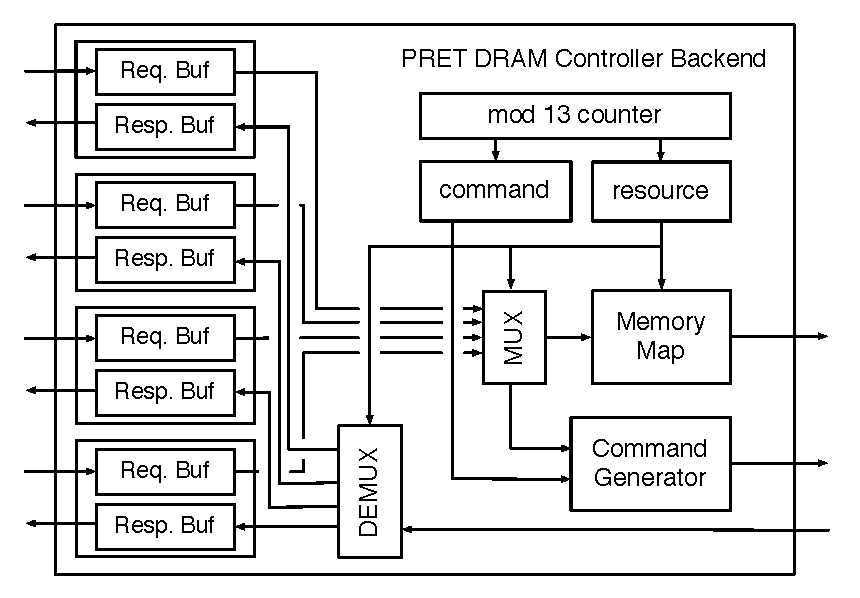
\includegraphics[width=1.1\linewidth]{figs/dram-backend-implementation}
\end{center}
\caption{Sketch of implementation of the backend~\cite{ReinekeLiuPatelKimLee11_PRETDRAMControllerBankPrivatizationForPredictability}.}
\label{fig:dram-backend-implementation}
\end{wrapfigure}

A high level block view of our backend implementation is shown in figure~\ref{fig:dram-backend-implementation}.
Each resource has a single request buffer and a respond buffer.
These buffers are used to interface with the frontend.   
A request is made of an access type (read or write), a logical address, and the data to be written for write requests. 
Requests are serviced at the granularity of bursts, i.e. 32 bytes in case of burst length 4 and 64 bytes in case of burst length 8.
A modulo-13 counter is used to implement the 13 cycle periodic access scheme in our controller.   
The ``resource'' and ``command" blocks are combinational circuits that are used to select the correct request buffer and generate the DRAM commands to be sent out. 
The ``memory map" block is where logical addresses are mapped to physical addresses that determine the rank, bank, row and column to access.
The data for read requests are latched into the response buffers to be read by the frontend.  

\paragraph{Frontend}
The frontend of our memory controller manages the interfacing to our backend, and the refreshing of the DRAM device.
The privatization of DRAM banks creates four independent resources that are accessed separately from the front end.
Thus, our memory controller is designed to be used by multicore or multithreaded architectures that contain multiple requesters which need access to the main memory.
Several recent projects, such as MERASA~\cite{Ungerer10}, PREDATOR~\cite{Akesson2007CODES}, JOP~\cite{Schoeberl2008265}, or CoMPSoC~\cite{Hansson09}, strive to develop predictable multi-core architectures that require predictable and composable memory performance.
These could potentially profit from using the proposed DRAM controller.

Specifically, we designed this memory controller to interface with the thread-interleaved pipeline discussed previously in section~\ref{section:pret_thread_pipeline}.
The thread-interleaved pipeline contains multiple hardware threads that each require access to main memory. 
We assign each hardware thread to a private memory resource, and send out memory requests to the memory controller frontend, which receives the request and places it within the request buffer.
Each thread in the thread-interleaved pipeline sends out only one outstanding memory request at a time, so the single request buffer for each resource is sufficient to interface with our thread-interleaved pipeline.
Once the request is serviced from the backend, the pipeline can read the data from the response buffer, and prepare to send another memory request.    
In section~\ref{sec:ptarm_memory} we will detail how our implemented thread-interleaved pipeline interfaces with this predictable DRAM controller, and discuss the memory access latency of this interaction.

\subparagraph{Shared Data}
The privatization of resources for predictable access means that there is no shared data in the DRAM.
This serves as an interesting design challenge, as it is impossible to assume no communication between contexts in a multicore or multithreaded environment.
In our implementation, which we will detail in section~\ref{sec:ptarm_memory}, the scratchpads can be configured to be shared between the hardware threads for communication.  
This can be done because the scratchpad and DRAM memory have distinct address regions, so no shared memory space will overlap onto the DRAM address space. 
%If conventional caches were used, which can cache
Most multi-core processors use DRAM to share data while local scratchpads or caches are private.
In this case, the sharing of data on the DRAM can be achieved by arbitrating accesses in the frontend.
The four independent resources in the backend can be combined into one, and any access to this single resource would result in four smaller accesses to all the backend resources. 
This single resource could then be shared among the different cores of a multi-core architecture using predictable arbitration mechanisms such as Round-Robin or CCSP~\cite{Akesson08} or predictable and composable ones like time-division multiple access (TDMA). 
This sharing of DRAM resources comes at a cost of increased memory access latency, which is detailed in~\cite{ReinekeLiuPatelKimLee11_PRETDRAMControllerBankPrivatizationForPredictability}. 

\subparagraph{Refreshing the DRAM}
The frontend of our memory controller also manages the refreshing of DRAM cells. 
DRAM cells need to be refreshed at least every 64 ms.
Conventionally this is done by issuing a hardware refresh command that refreshes several rows of a device at once\footnote{Internally, this still results in several consecutive row accesses.}.
Hardware refresh commands have longer refresh latencies each time a refresh is issued, but require fewer refresh commands to meet the refresh constraints posed by the DRAM.
However, when the hardware refresh command is issued, all banks in the target DRAM device are refreshed, prohibiting any other memory access to the device.
In our backend, this would extend across multiple resources, causing multiple resources to be blocked for memory accesses. 
Memory access latencies now need to account for potential refresh command latencies, which vary depending on the refresh progress.  
Instead, we use the distributed, RAS-only refresh~\cite{spec:micronddr2} to each bank separately.
Memory refreshes in this case are equivalent to row accesses to a bank; each resource can be refreshed without effecting others.
Manually accessing rows on the other give much shorter latencies each time, but incur a slight bandwidth hit because more accesses need to be performed to meet the refresh constraints.
The shorter latencies however improve the worst-case access latency, because the refresh latency is shorter.

%When a refresh is required can be statically analyzed. 
In our device, each bank consists of 8192 rows, so each row has to be refreshed every $64\textit{ms}/8192=7.8125 {\mu}s$.
At a clock rate of 200 MHz of the memory controller, this corresponds to $7.8125 {\mu}s \cdot (200 \textit{cycles}/{\mu}s) = 1562.5$ cycles.
Since each resource contains two banks, we need to perform two refreshes every $1562.5$ cycles, or one every $781.25$ cycles.
One round of access is $13$ cycles at burst length 4, and includes the access slots to each resource plus a nop command. 
So in the frontend we schedule a refresh every $\lfloor 781.25/13 \rfloor^{th} = 60^{th}$ round of the backend.
If no memory access is in the request buffer for the resource being scheduled for refresh, then the row refresh can be directly be issued. 
Conventionally, when a contention between a memory request and a refresh occurs, the refresh gets priority so the data can be retained in the DRAM cell. 
However, our refresh schedule schedules refreshes slightly more often than necessary.   
Scheduling a refresh every $60 \cdot 13$ cycles means that every row, and thus every DRAM cell, is refreshed every $60\cdot 13 \textit{ cycles}\cdot 8192\cdot 2/(200000~\textit{cycles}/\textit{ms}) \leq 63.90\textit{ms}$.
We can thus push back any of these refreshes individually by up to $0.1\textit{ms} = 20000$ cycles without violating the refreshing requirement.
So in our frontend, the memory request is serviced first (which takes 13 cycles), then the refresh is issued in the next access slot. 

In section~\ref{sec:ptarm_memory} when we detail the interaction between our thread-interleaved pipeline and the memory controller, we will show that the synchronization of the thread-interleaved pipeline to our controller backend allows us to completely hide memory refreshes in some unusable access slots lost in the synchronization.
This provides predictable access latencies for all load/store instructions to the DRAM through our DRAM controller.

%\todo{discuss DMA?}
%We will also discuss interactions with DMA units    
%For loads sent from the pipeline, the pushed back refreshes become invisible:
%as the pipeline is waiting for the data to be returned and takes some time to reach the memory stage of the next instruction, it is not able to use successive access slots of the backend, and thus it is unable to observe the refresh at all.
%With this refresh scheme, refreshes do not affect the latencies of load/store instructions, and the refreshes scheduled within DMA transfers are predictable so the latency effects of the refresh can be easily analyzed.




\section{Programming Models}
\label{chapter:programming_models}
Intro text here

\subsection{PRET Programming model Section Header}
\label{sec:pret_prog_model_sec_1}

\subsection{Pret Programming model Section Header 2}
\label{sec:pret_prog_model_sec_2}

Here is another header


